%!TEX root = ../data-imputation.tex
\section{Results}
\label{sec:results}

In this section, we describe and visualize the results of our experiments. For the visualization we choose to use box plots for all four experiments/scenarios. These allow us to get a decent impression of the distribution of the results based on quantiles. In a line chart, in contrast, the confidence bands would overlap too much to derive meaningful interpretations. The plots' arrangement from left to right corresponds to the degree of difficulty increasing in this direction. This applies to the missingness patterns (MCAR, MAR, MNAR), each of which gets a subplot, as well as the missingness percentages (small to larger), which are depicted as ticks on the x-axis. To show different effects of imputing categorical or numerical columns, we split the plots horizontally. Because we randomly sample on target column for each data set, there are about $13\%$ categorical ($9$) and $87\%$ numerical ($60$) columns. Respectively, for the second experiment, the horizontal split presents classification and regression downstream tasks, which are also imbalanced: $48$ classification ($\sim70\%$) and $21$ regression tasks ($\sim30\%$).

\subsection{Experiment 1: Imputation Quality}

In this experiment we evaluate the imputation performance of each method when training on complete data. As described above, our goal was to provide a broad overview of the imputation methods' performance on various data sets. Using randomly sampled target columns on heterogeneous data leads to a wide range of values for their evaluation metric ($F1$/$RMSE$), which makes it difficult to compare. To aggregate results across such heterogeneous sets of metrics, we split the results in categorical and numerical imputation and compute the rank of each imputation method for every missingness pattern and fraction separately. Since we use six imputation methods, there are six ranks, where rank one is best and rank six the worst. If two or more methods perform equally, we assign the same rank and for methods that failed during training rank six.


\subsubsection{Scenario 1: Training on Complete Data}
\label{sec:results_experiment1_scenario1}

\begin{figure}\centering
    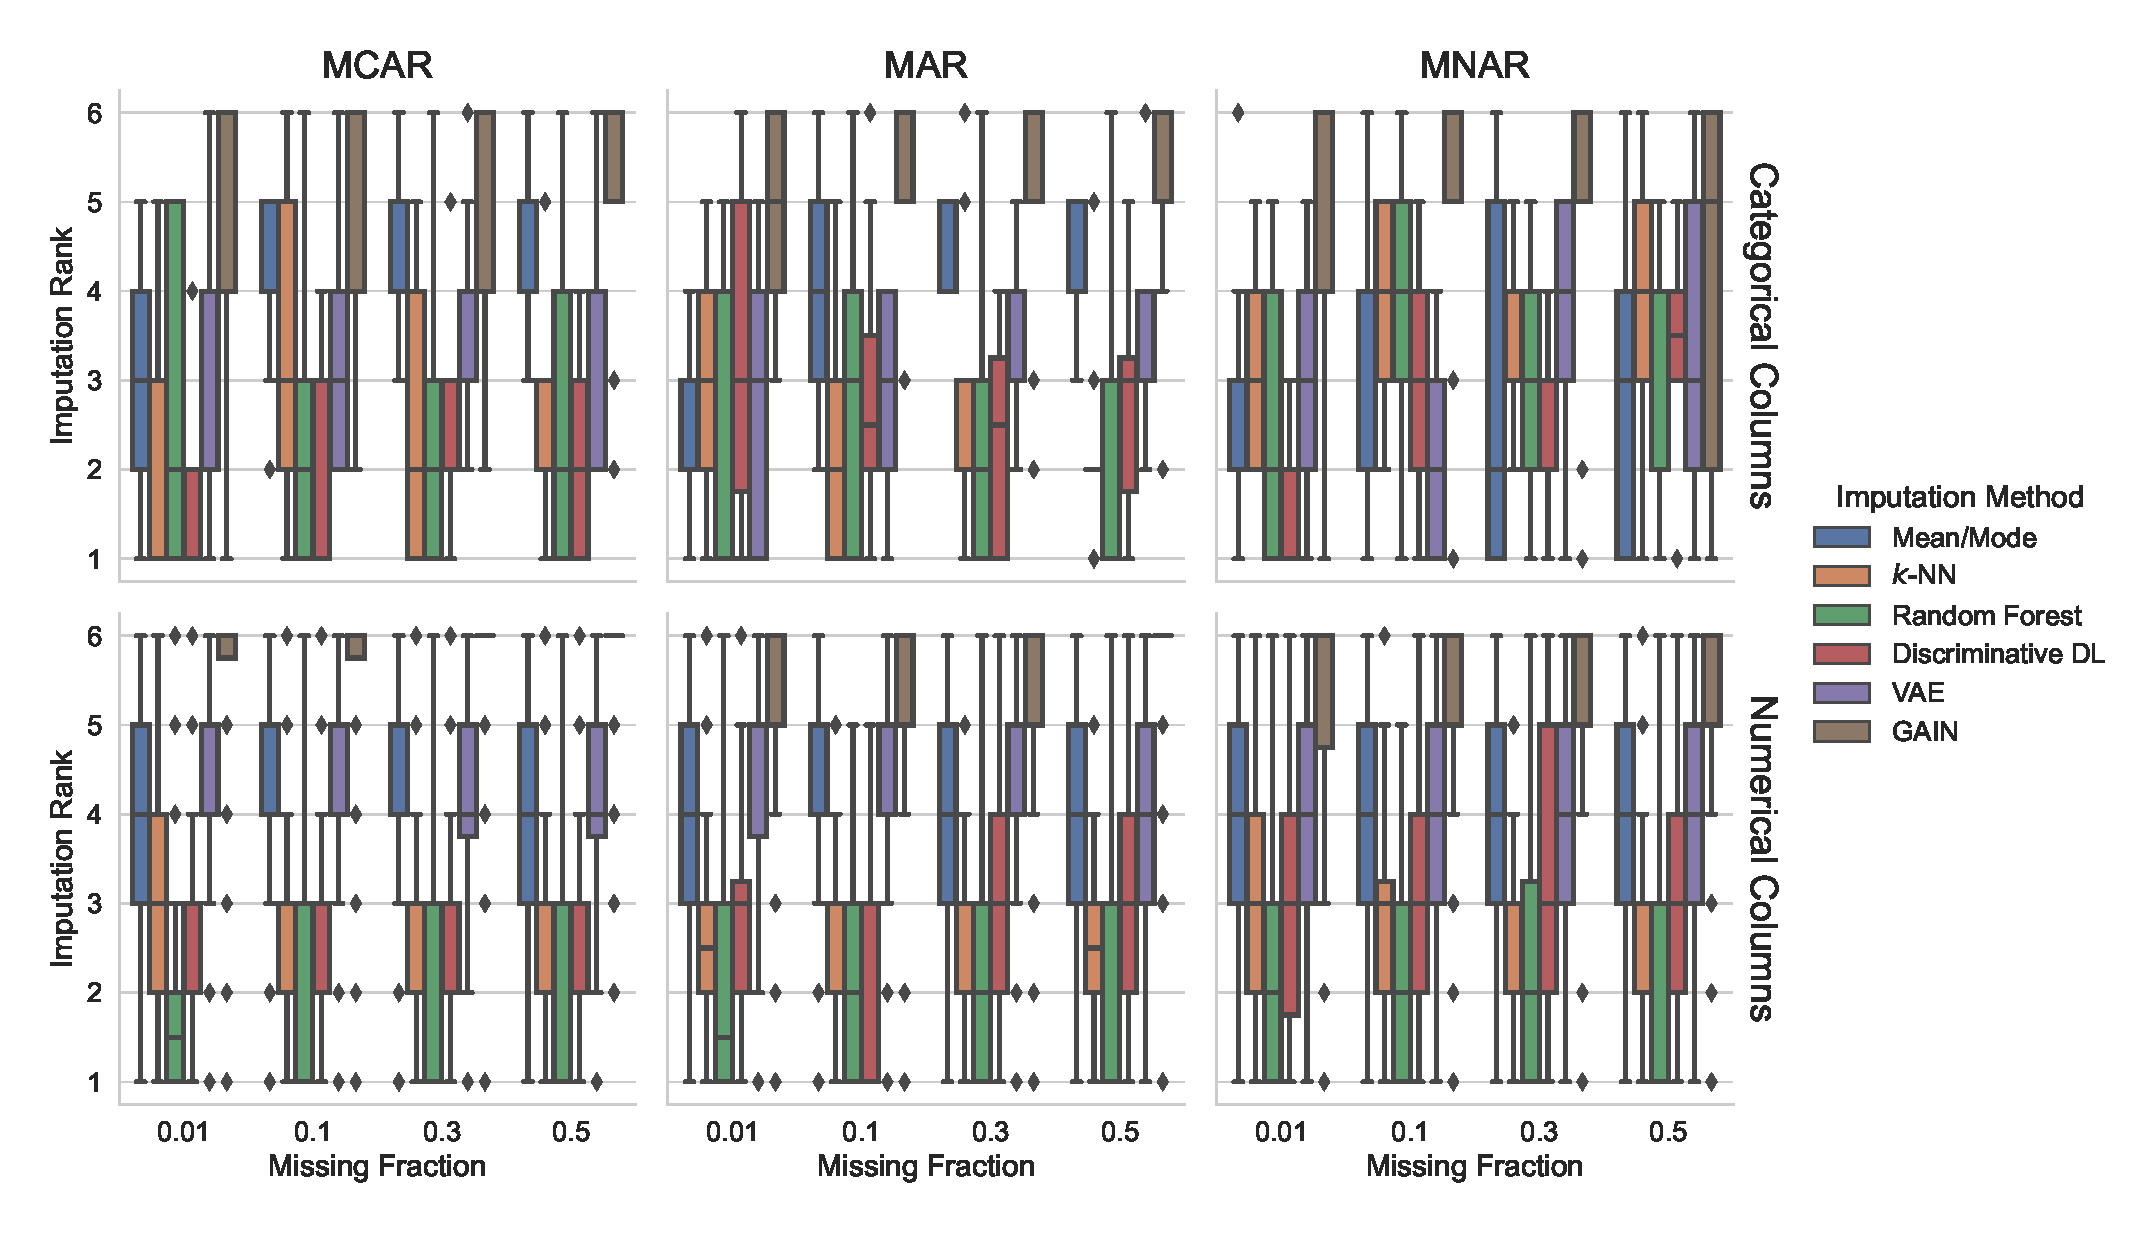
\includegraphics[width=1\columnwidth]{fully_observed_impute_rank_boxplot.eps}
    \caption{Imputation ranks of the  imputation methods trained on complete data. Ranks are computed for each experimental condition characterized by datat set, missingness pattern and missingness ratio. In most conditions random forest, $k$-NN and discriminative DL perform best. Generative Deep Learning methods tend to perform worst. In the most challenging MNAR condition mean/mode imputation achieves competitive results.
	}
	\label{fig:fully_observed_impute_rank_boxplot}
\end{figure}


Figure \ref{fig:fully_observed_impute_rank_boxplot} presents the imputation results when training on complete data. In about $33\%$ of these results, GAIN failed during training and get assigned the worst rank six.

When imputing categorical columns, there is no clear best method. However, in many settings the discriminative DL approach achieves for $75\%$ of the cases at least rank three or better. Very similar but slightly worse results are shown by the random forest imputation method. For MCAR with $50\%$ missing values and MAR with $10\%$ to $50\%$ missingness, the $k$-NN imputation approach performs well and gets for $75\%$ of the cases at least rank three or better. VAE achieves in $50\%$ of the cases a rank between two and four, and GAIN shows consistently the worst performance, in most settings it is placed fourth or worse in $75\%$. Interestingly, mean/mode imputation scores better ranks for the more complex settings with MNAR missingness pattern.

When imputing numerical columns, the differences are more pronounced. Random forest is the only method that achieves one of the first three ranks in $75\%$ of the cases throughout all experimental conditions. Also $k$-NN shows good results, ranking second or third in most settings in $50\%$ of the cases. Very similar results are achieved by the discriminative DL method that tends to lose performance from MAR with $30\%$ missingness to MNAR with $50\%$ missing values. Again VAE ranges most of the time between rank three and five similar to mean/mode imputation and GAIN gets the worst ranks five and six.

To summarize, simple imputation methods, such as $k$-NN and random forest, often perform best, closely followed by the discriminative DL approach. However, for imputing categorical columns with MNAR missing values mean/mode imputation often performs well, especially for high fractions of missing values. The generative approaches get middle ranks (VAE) or range on the worst ranks (GAIN).

\subsubsection{Scenario 2: Training on Incomplete Data}


\begin{figure}\centering
    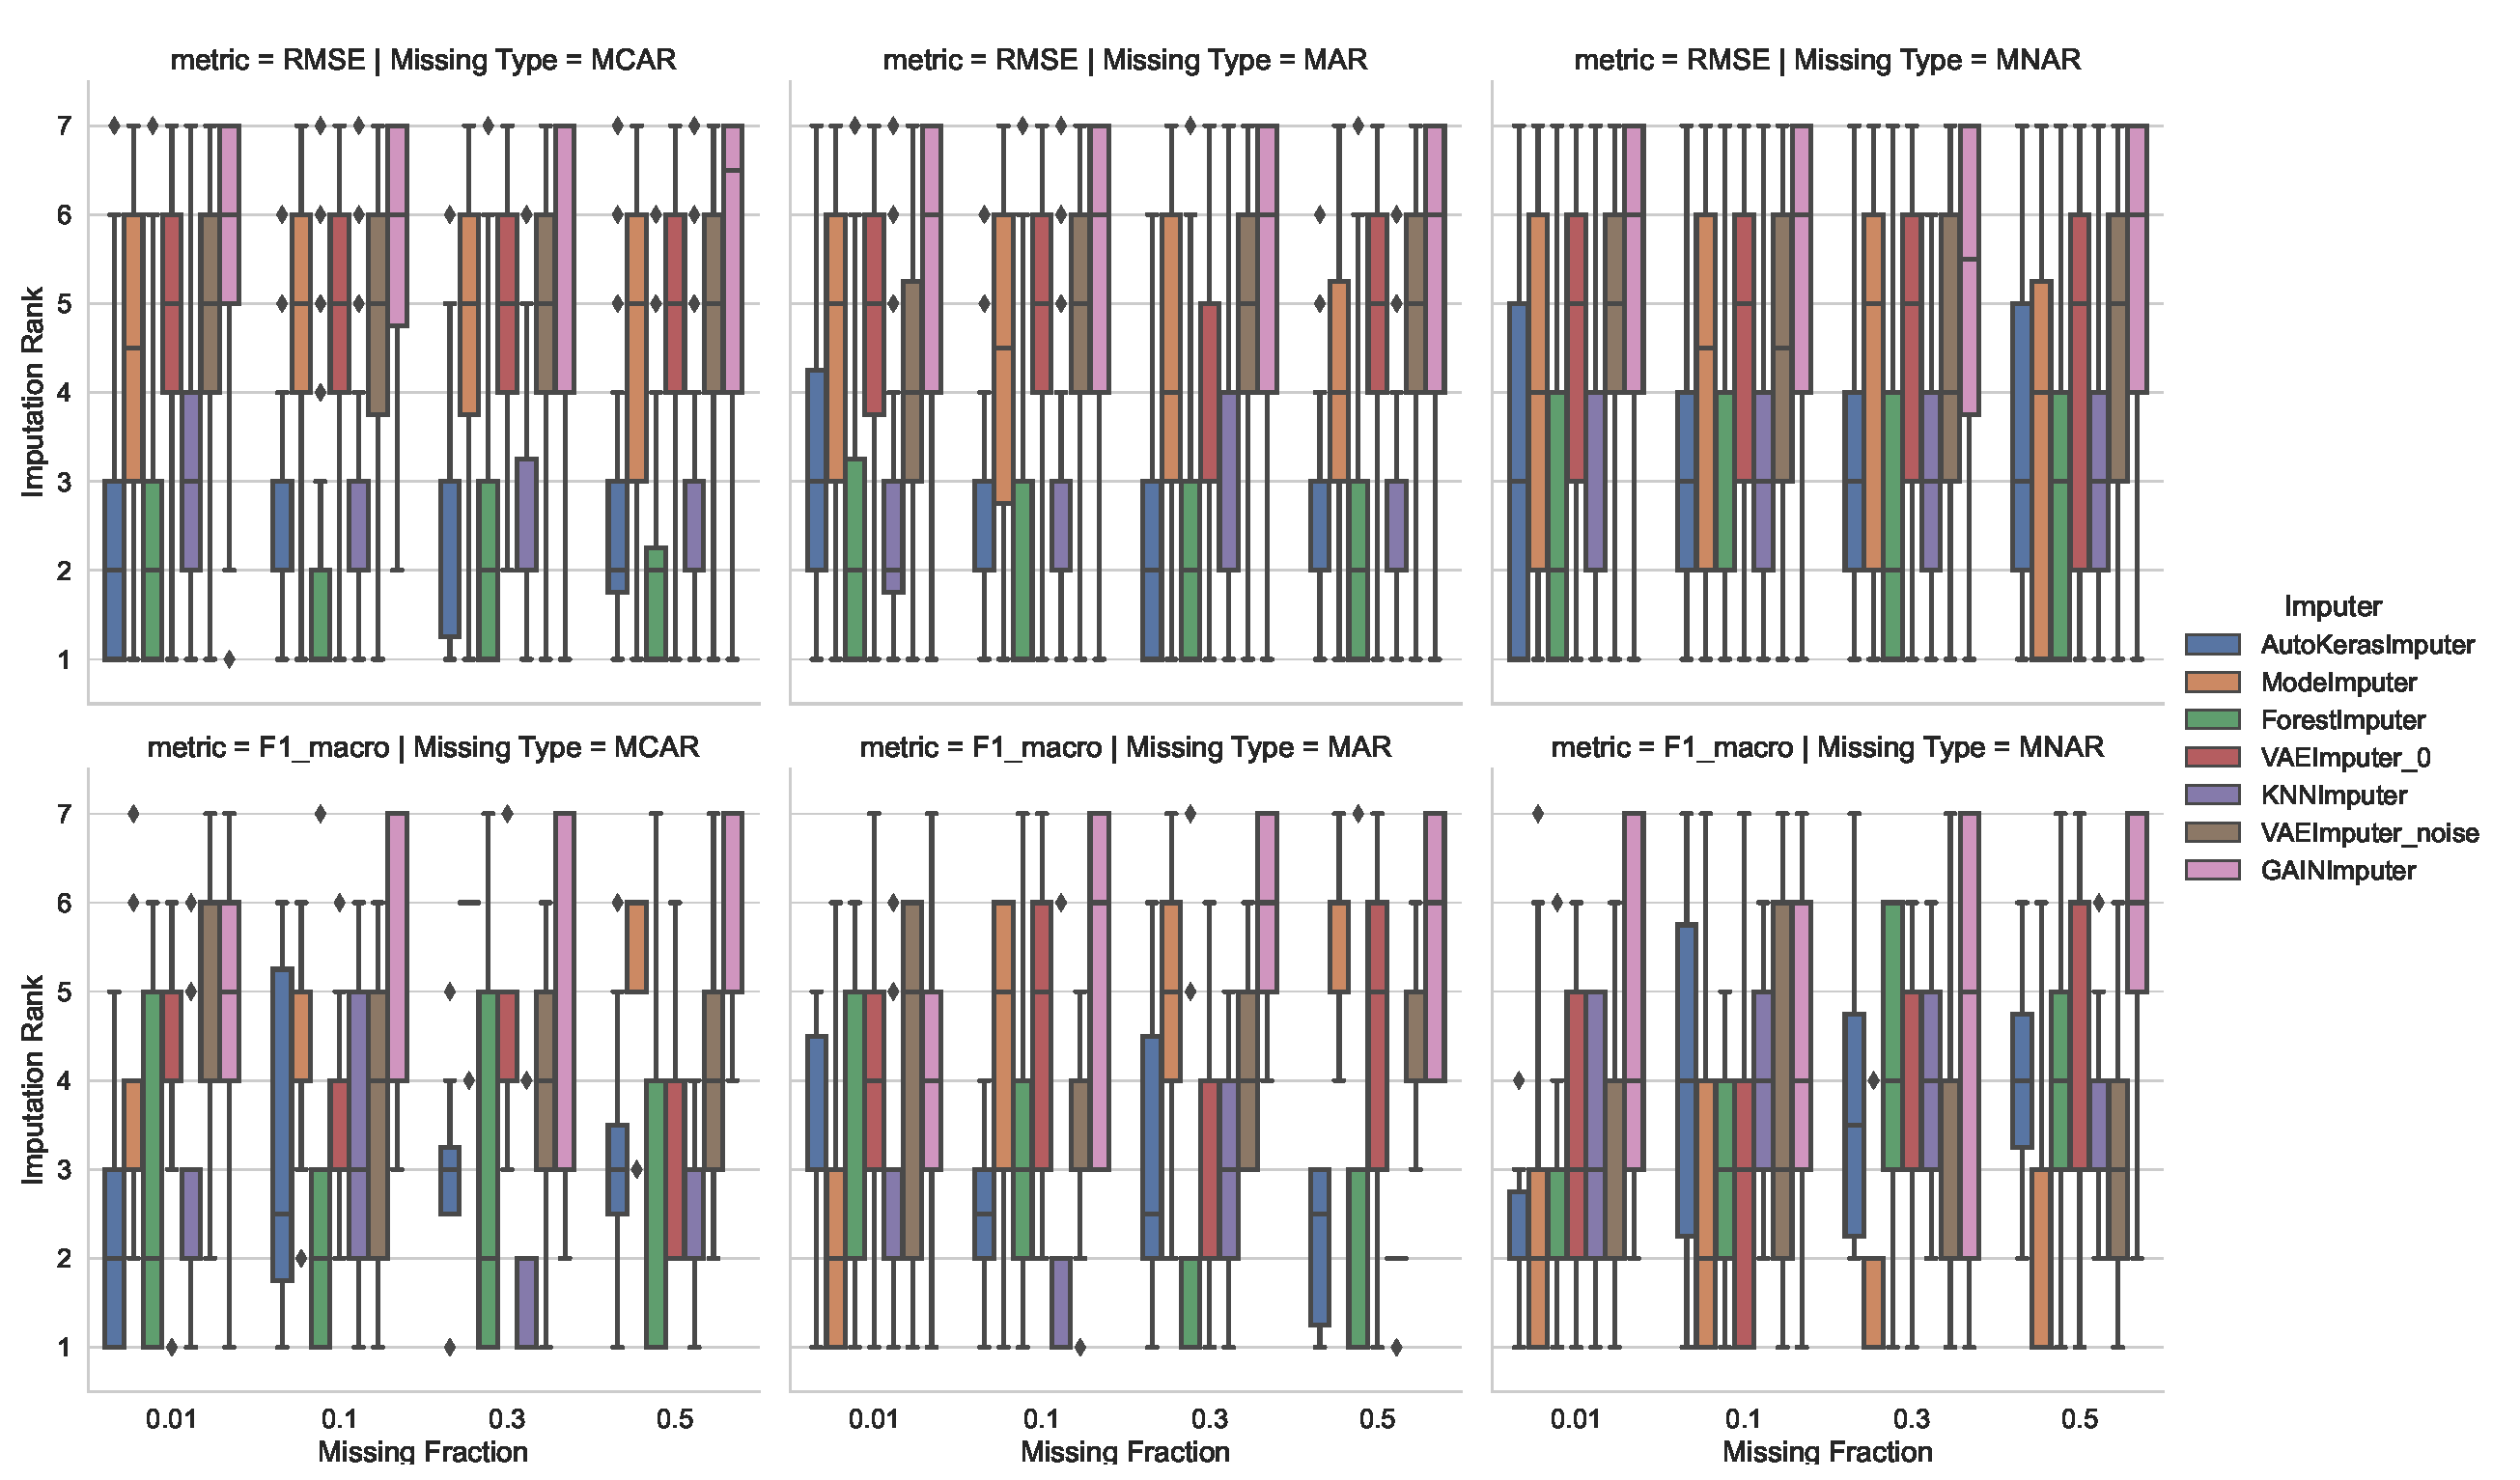
\includegraphics[width=1\columnwidth]{corrupted_impute_rank_boxplot.eps}
    \caption{Imputation ranks of the  imputation methods trained on {\em incomplete} data. Ranks are computed for each experimental condition characterized by datat set, missingness pattern and missingness ratio. Similar to the training on fully observed data random forest, $k$-NN and discriminative DL perform better than generative Deep Learning methods in most settings. In the MNAR conditions, the imputation quality of all imputation approaches degrades in favor of mean/mode that clearly outperforms the other for $30\%$ and $50\%$ missingness.}
	\label{fig:corrupted_impute_rank_boxplot}
\end{figure}

\autoref{fig:corrupted_impute_rank_boxplot} shows the imputation performance in \textit{Scenario 2}, i.e., when training on incomplete data. Imputing categorical columns with increasing difficulty, the ranks of mean/mode imputation improves. From MCAR $30\%$ to MNAR $50\%$, $k$-NN is in $75\%$ of the cases on at least the third rank or better, often it ranges on the first and second rank. For MNAR its performance degrades gradually in favor of mean/mode that shows surprisingly good results, especially for the most challenging settings (MNAR with $30\%$ and $50\%$ missing values) where it clearly outperforms others in at least $75\%$ of the cases. Random forest has very high variance but on most missingness fractions with MCAR pattern, it ranks in $50\%$ of the cases on rank two or better. For MNAR its rank improves with higher missingness fractions, whereas this trend reverses for MAR. In most cases, the generative methods rank worst (GAIN) and on the middle ranks (VAE). However, with high missingess and when missing values are MNAR, they can perform better.

Similar to the fully observed training case (Section \ref{sec:results_experiment1_scenario1}), imputation on numerical columns yields a clearer ranking than for categorical missing values. The imputation methods $k$-NN and random forest rank best with a tendency of random forest to outperform $k$-NN, where random forest's variance is higher. The discriminative DL approach yields very similar performance to the $k$-NN for MCAR and MAR settings. In the more challenging MNAR setting, it ranks slightly worse. For MCAR, mean/mode imputation ranks in almost all settings in $50\%$ of the cases between rank four and five, for MAR and MNAR between rank three and five. Again the generative methods rank in almost all settings in $75\%$ of the cases worse than rank for, where VAE tends to seldom rank the worst rank six.

Overall, the results of \textit{Scenario 1} (Figure \ref{fig:fully_observed_impute_rank_boxplot}) and \textit{Scenario 2} (Figure \ref{fig:corrupted_impute_rank_boxplot}) for numerical columns are quite similar. GAIN has become better in Scenario 2, although it still ranks worst. For categorical the ranks show generally higher variance. Most imputation methods getting worse with higher difficulty of the experimental setting, especially for MNAR, expect of mean/mode, which ranks better for MNAR. This effect is even clearer when training on incomplete data. In general, using simpler methods, such as $k$-NN or random forest, achieves good to best results in most settings and cases.


\subsection{Experiment 2: Impact on Downstream Task}

In this experiment, we evaluate the imputation method's impact on the downstream performance in two scenarios: the imputation model was trained on complete and incomplete data. As described in Section \ref{sec:experiment_2}, this time, we discard only values in the data set's randomly sampled target column. We exclude the experiment setting, which failed during training the imputation model, i.e., there are about $33\%$ fewer results for the first scenario (training on complete data).


\subsubsection{Scenario 1: Training on Complete Data}

\begin{figure}\centering
	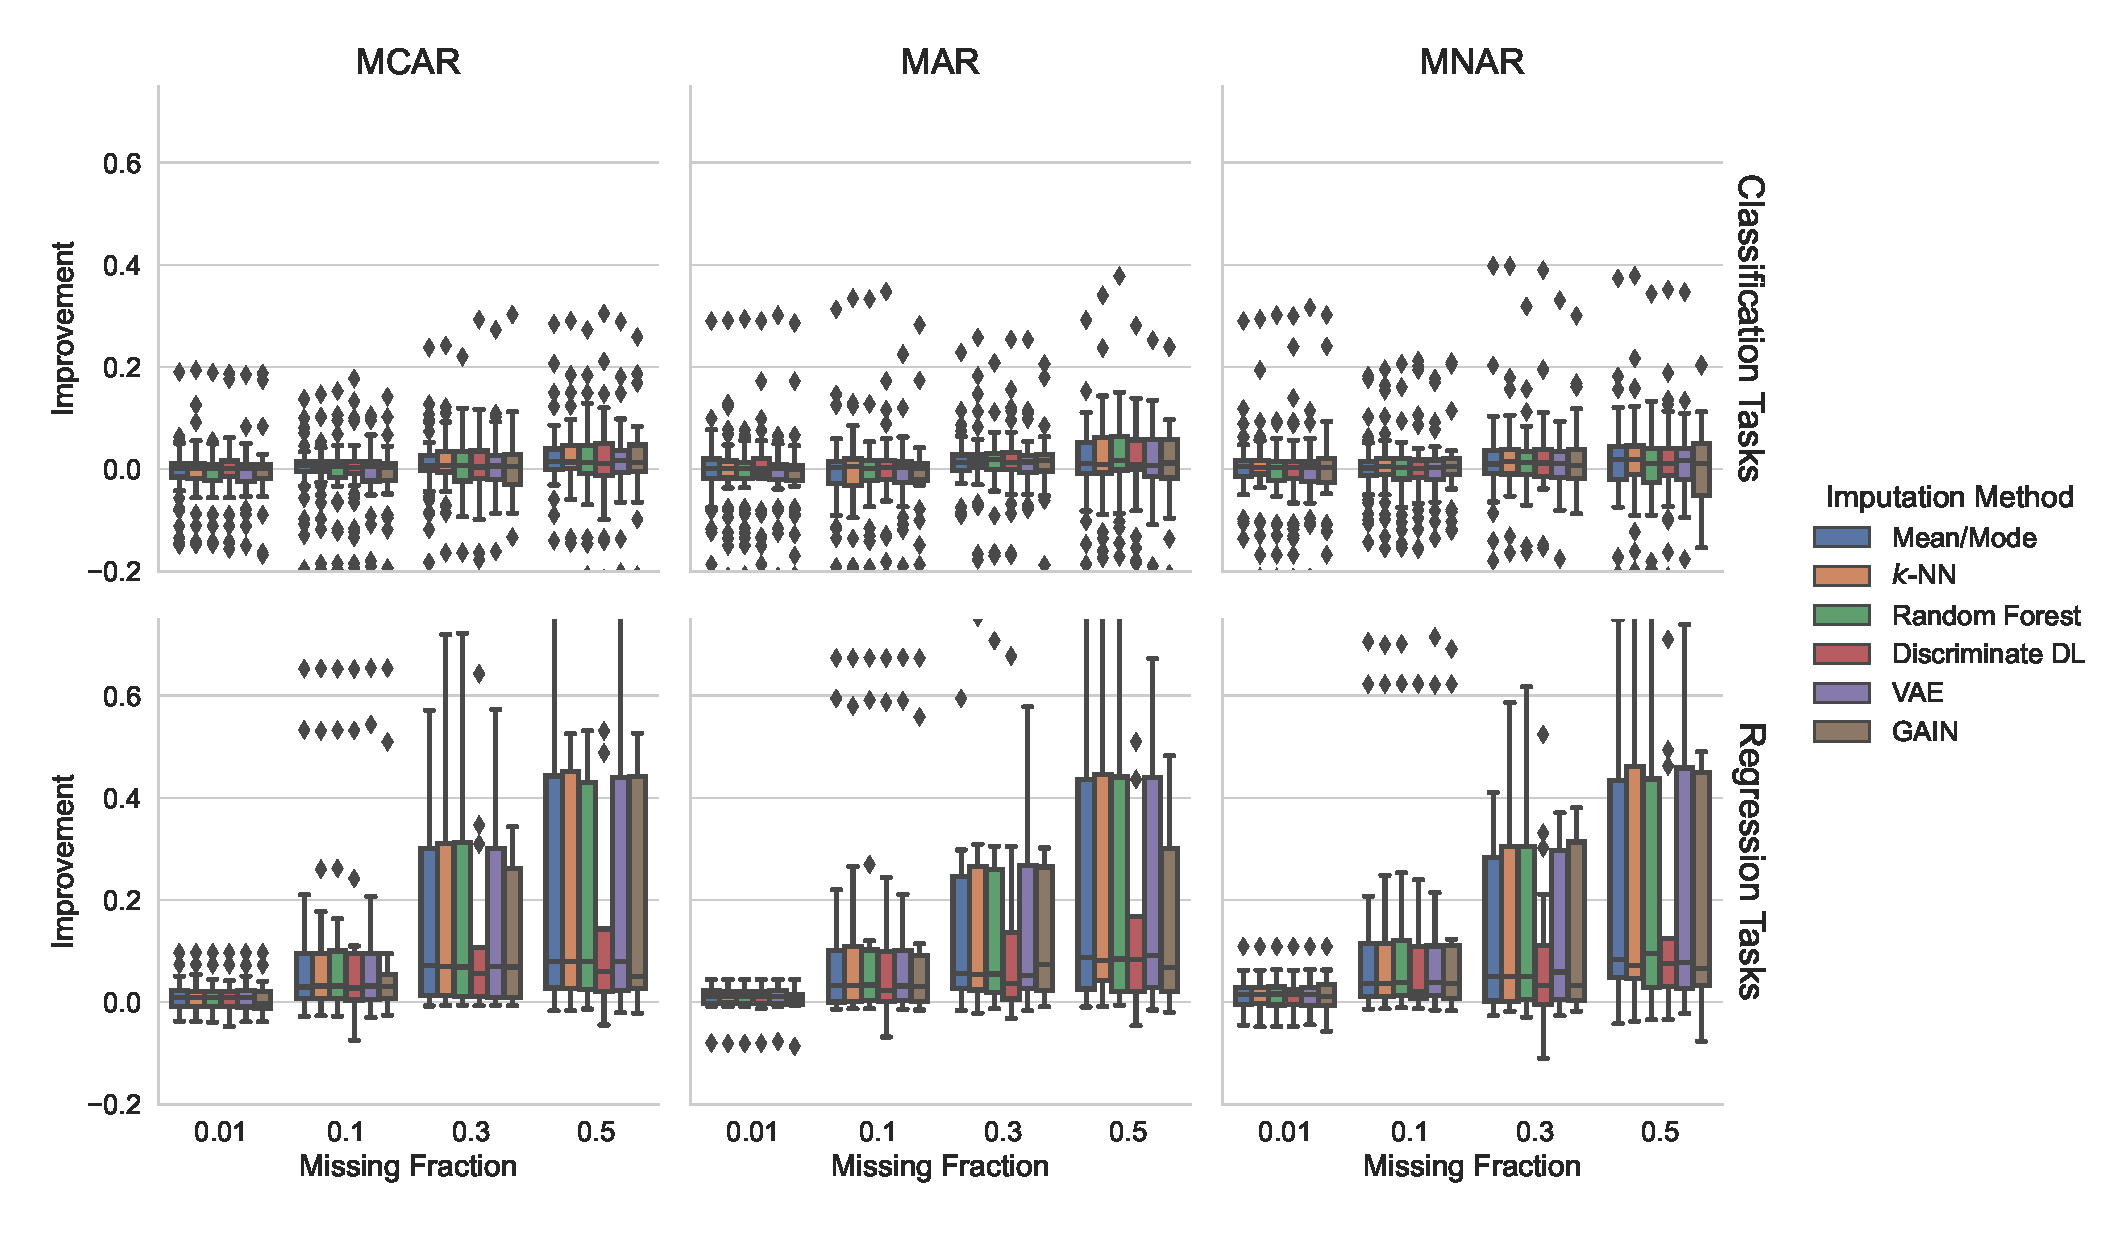
\includegraphics[width=1\columnwidth]{fully_observed_downstream_boxplot.eps}
	\caption{Does imputation on incomplete test data improve predictive performance of a downstream ML model? We plot the improvement of the downstream ML model after imputation with imputation models trained on fully observed data. The downstream performance is compared to the performance obtained on incomplete test data, normalized by the ML model performance on fully observed test data. Overall, the classical ML methods and discriminative DL perform best achieving relative improvements of up to 10\% and more relative to fully observed test data.
    }
	\label{fig:fully_observed_downstream_boxplot}
\end{figure}

Figure \ref{fig:fully_observed_downstream_boxplot} visualizes how much the predictive performance of a downstream ML model improves compared to incomplete test data and normalize by the downstream performance obtained on fully observed test data (Equation \ref{eq:impact}). This metric is labeled \textit{Improvement} and represented on the plots' y-axis.

In all cases, using imputation approaches increase the downstream performance in $75\%$ of the cases. Not surprisingly, independent from the downstream task and the missingness pattern, the more missing values exist, the better the potential improvement, shown by the method's increasing median and $75\%$ quantile.

For regression tasks, all imputation methods on all settings degrade the performance in less than $25\%$ of the cases. Further, they hold great potential for improving the performance in the range of $\sim10\%$ and $\sim15\%$ for $30\%$ and $50\%$ MCAR or MAR missing values. However, there is a tendency from MCAR to MNAR that the potential performance degrades. In most settings, random forest's median improvement is best, followed by $k$-NN and discriminative DL. This effect also holds for their potential improvement ($75\%$ quantile), except for $50\%$ MNAR, where it is about five percentage points higher than the others. In most settings, VAE and mean/mode increase the downstream performance very similar but worse than the other three, and GAIN is always the worst.

For classification tasks, few imputation methods in some settings show degrading performance in slightly more than $25\%$ of the cases. However, their median imputation performance is always positive and generally higher than for regression tasks. In general, the potential improvements of the methods are in all settings roughly the same. As for regression tasks, random forest, followed by $k$-NN and discriminate DL, hold in $50\%$ of the cases the best performance. Unfortunately, this degrades from MCAR to MNAR. Surprisingly, this time GAIN holds much more potential improvement and performs in many settings better than VAE, especially when the missingness fraction is high.

All in all, independent from the experimental settings, random forest performs in $50\%$ of the cases best, closely followed by $k$-NN and discriminative DL. In general, when using imputation, the expected improvement is for classification higher than for regression tasks. This effect also holds for the missingness fractions: the higher the missingness fraction, the higher the potential improvements. Only in less than $25\%$ of all cases, we found degraded downstream performance.


\subsubsection{Scenario 2: Training on Incomplete Data}

\begin{figure}\centering
	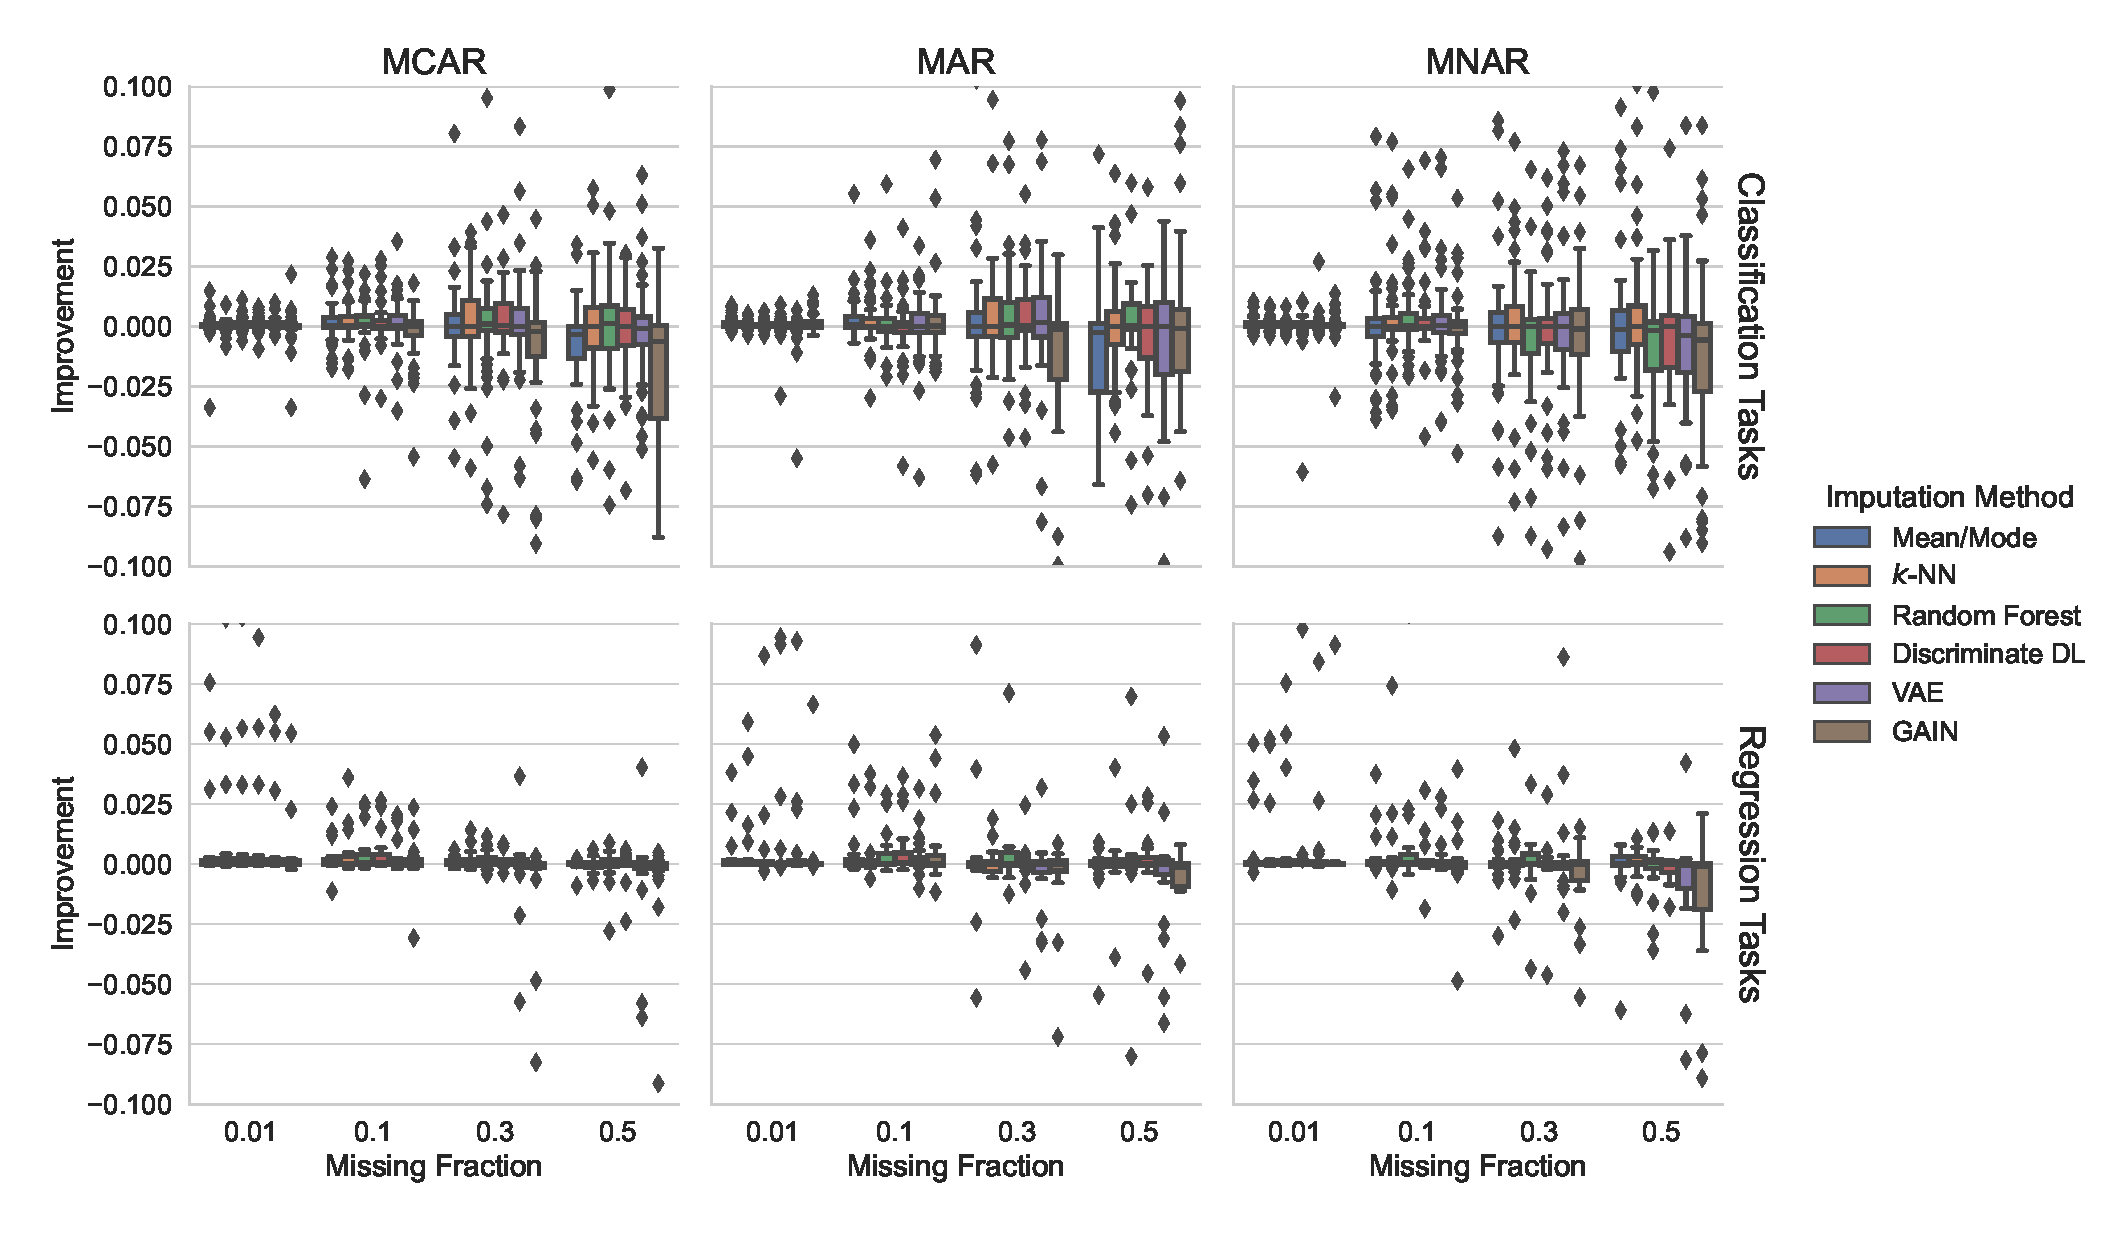
\includegraphics[width=1\columnwidth]{corrupted_downstream_boxplot.eps}

	\caption{Impact on downstream task of the six imputation methods trained on incomplete data. In regression tasks, no considerable improvements are achieved, in some cases imputation actually worsened the downstream ML model. In classification tasks, in contrast, we observe slightly positive effects in some settings but negative effects predominate in the harder settings.
    }
	\label{fig:corrupted_downstream_boxplot}
\end{figure}


Figure \ref{fig:corrupted_downstream_boxplot} illustrates the impact imputation has on the downstream task. We show how many percent the predictive performance of a downstream ML model improves compared to incomplete test data. This metric is labeled \textit{Improvement} and represented on the plots' y-axis. Here, the different scaling must be taken into account, i.e., the relative improvements are considerably smaller compared to the first scenario. One reason for this is the different basis for calculating the relative values (see Sections \ref{sec:experiment_2} and \ref{sec:scenario_2}).

The potential improvements when the imputation methods are trained on incomplete data are marginal. In all settings, there are hardly any improvements greater than $1\%$. However, with $30\%$ missing values or fewer, most cases have a positive impact.

For classification tasks, with up to $30\%$ MCAR or MAR missingness, there for all imputation methods, but GAIN, mostly very small but positive improvements, where higher missing fractions yield potentially higher improvements ($75\%$ quantile). However, high missingness fractions shift the improvements into the negative range, i.e., degrade the performance. For MNAR only for $1\%$ and $10\%$ missing values, we see mostly improvements, and for $30\%$ or $50\%$ missingness, the downstream performance degrades in most cases.

For regression tasks, there are hardly any potential improvements over $0.5\%$. On the other hand, there are also much fewer cases where imputation potentially degrades the performance. Outstanding is random forest, which yields in most settings the highest performance and the generative approaches that harm the performance when missingness is $30\%$ or higher.

To summarize, for up to $30\%$ missing values independent of the missingness pattern or downstream tasks, imputation increases the performance in most cases. Using random forest holds the best chance in almost all settings to improve the downstream performance.

\subsection{Computational Complexity}
%
Our results demonstrate that simple ML methods are often on par with modern deep learning methods. An important question in this context is how the various methods compare in terms of their computational complexity: if methods yield similar predictive performance, it is preferable to use those alternatives with the least computational effort. To measure the training and inference time, we use a sub-set of our experiments. Precisely, all data sets, missingness fractions and imputation methods (shown in Table \ref{tab:experiment_settings}) with MCAR pattern. We first train the imputation method on complete data, then discard values of the given missingness fraction in the training set, and impute those missing values. The wall-clock run time is measured in seconds when calling our framework's \code{fit} and \code{transform} methods (see Section \ref{sec:implementation} for details), which means that the training duration incorporates the hyperparameter optimization (see Section \ref{sec:HPO} for details).

Because training and inference time depend heavily on the data set's size, directly average all experiments for the imputation methods lead to very similar mean but extremely high standard deviation values. For this reason, we first compute the mean duration and the standard deviation relative to its mean separately for training and inference for the imputation methods on each data set. Second, we average those values for each imputation method and present them in Table \ref{tab:time}. Using this approach helps to average over all experiments, and, at the same time, gives indicators for the training and inference durations, as well as their variance.
%
\begin{table}
	\centering
	\begin{tabular}{@{\extracolsep{4pt}}lrrrr@{}}
		\toprule
		\multirow{2}{*}{Imputation Method} & \multicolumn{2}{c}{Training} & \multicolumn{2}{c}{Inference} \\\cline{2-3}\cline{4-5}
		\\[-0.75em]
		& Mean Duration &   Rel. SD & Mean Duration &   Rel. SD \\
		\midrule
		Mean/Mode &      0.005 &  0.550 &      0.029 &  0.171 \\
		\\[-0.5em]
		$k$-NN &     41.204 &  0.254 &       7.018 &  0.602 \\
		\\[-0.5em]
		Random Forest &    226.077 &  0.119 &     24.048 &  0.236 \\
		\\[-0.5em]
		Discriminative DL &   6275.019 &   0.405 &    440.389 &  0.211 \\
		\\[-0.5em]
		VAE &     71.095 &  0.099 &      11.215 &  0.085 \\
		\\[-0.5em]
		GAIN &    878.058 &  0.312 &     137.966 &  0.083 \\
		\bottomrule
	\end{tabular}
	\caption{Training and inference duration for each imputation method in seconds. We use the wall-clock run time to measure the durations for training, including hyperparameter optimization, and inference for all data sets with MCAR missingness pattern and all fractions shown in Table \ref{tab:experiment_settings}. Because training and inference durations depend heavily on the data set size, we first calculate the durations' mean and relative standard deviation for each imputation method on every data set. Second, we average those mean durations and relative standard deviations for the imputation methods and present them as \emph{Mean Duration} and \emph{Rel. SD} separately for \emph{Training} and \emph{Inference}. Abbreviations: \emph{Rel. SD} means Relative Standard Deviation.
	}
	\label{tab:time}
\end{table}

As expected, if the imputation model's complexity increases, their training duration increases too, most of the time by multiple factors. There are two exceptions: discriminative DL and VAE, an explanation for this could be their number of hyperparameter combinations optimized during training. VAE optimizes only three, GAIN $16$, and discriminative DL $50$ combinations, which represents their training durations order.

Similarly, the inference time increases with the model's complexity. The differences are clear but not as high as for the training durations.
Higher inference standard deviations, e.g., for $k$-NN and random forest (and discriminative DL), indicate that the found best hyperparameters strongly varying with the experimental settings and influence the model's computational complexity for inference. One reason for the discriminative DL's and GAIN's high training standard deviations could be the usage of early-stopping and, at the same time, indicate that it is important to try a huge number of hyperparameters to achieve good results. For mean/mode the high standard deviation is likely an artifact of the very small training duration. Changes in milliseconds for computations are common and represent a large change relative to the mean/mode imputation's mean duration.

To summarize, the increasing complexity of the imputation methods are clearly represented in their training and inference duration. For training more complex models, this is supported by higher variance of training time indicating the necessity to try a wide range of hyperparameters. On the other hand, once found, the hyperparameters  for generative models influence the inference time less than for $k$-NN or random forest, which prediction times depend heavily on the hyperparameters.
